\documentclass[fleqn, a4paper, 11pt, oneside]{amsart}
\usepackage{exsheets}
\usepackage{amsmath, amssymb, amsthm} %standard AMS packages
\usepackage{marginnote} %marginnotes
\usepackage{gensymb} %miscellaneous symbols
\usepackage{commath} %differential symbols
\usepackage{xcolor} %colours
\usepackage{cancel} %cancelling terms
\usepackage[free-standing-units, space-before-unit]{siunitx} %formatting units
\usepackage{tikz, pgfplots} %diagrams
	\usetikzlibrary{calc, hobby, patterns, intersections, decorations.markings}
\usepackage{graphicx} %inserting graphics
\usepackage{hyperref} %hyperlinks
\usepackage{datetime} %date and time
\usepackage{enumerate,enumitem} %numbered lists
\usepackage{float} %inserting floats
\usepackage{circuitikz}[american voltages, american currents] %circuit diagrams
\usepackage{booktabs}
\usepackage{csvsimple}

\newcommand\numberthis{\addtocounter{equation}{1}\tag{\theequation}} %adds numbers to specific equations in non-numbered list of equations

\theoremstyle{definition}
\newtheorem{example}{Example}
\newtheorem{definition}{Definition}

\theoremstyle{theorem}
\newtheorem{theorem}{Theorem}

\makeatletter
\@addtoreset{section}{part} %resets section numbers in new part
\makeatother

\SetupExSheets{solution/print = true}

%opening
\title
[
	Introduction to Signal Analysis : Assignment 1
]
{
	Introduction to Signal Analysis\\
	Assignment 1
}
\author
{
	Aakash Jog\\
	ID : 989323563
}
\date{\formatdate{23}{3}{2016}}

\begin{document}

\maketitle
%\setlength{\mathindent}{0pt}

\begin{question}
	Sort the following systems based on linearity, time invariance, memory, causality, invertibility, and stability.
	\begin{enumerate}
		\item $y(t) = 1 + x(t) \cos(\omega t)$
		\item $y(t) = \sum\limits_{n = -\infty}^{\infty} x(t) \delta(t - n T)$
		\item $y(t) = \int\limits_{-\infty}^{\infty} \sin(t + \tau) x(\tau) \dif \tau$
	\end{enumerate}
\end{question}

\begin{solution}
	\begin{enumerate}[leftmargin=*]
		\item
			\begin{enumerate}
				\item
					\begin{align*}
						H\left\{ x(t) \right\} & = y(t) \\
                                                                       & = 1 + x(t) \cos(\omega t)
					\end{align*}
					Therefore,
					\begin{align*}
						H\left\{ a x_1(t) + b x_2(t) \right\} & = 1 + \left( a x_1(t) + b x_2(t) \right) \cos(\omega t) \\
                                                                                      & = 1 + a x_1(t) \cos(\omega t) + b x_2(t) \cos(\omega t) \\
                                                                                      & \neq a H\left\{ x_1(t) \right\} + b H\left\{ x_2(t) \right\}
					\end{align*}
					Therefore, the system is non-linear.
				\item
					\begin{align*}
						H\left\{ x(t) \right\} & = y(t) \\
                                                                       & = 1 + x(t) \cos(\omega t)
					\end{align*}
					Therefore,
					\begin{align*}
						H\left\{ x(t - t_0) \right\} & = 1 + x(t - t_0) \cos(\omega t) \\
                                                                             & = 1 + x(t - t_0) \cos(\omega t) \\
                                                                             & \neq y(t - t_0)
					\end{align*}
					Therefore, the system is time-variant.
				\item
					\begin{align*}
						y(t) & = 1 + x(t) \cos(\omega t)
					\end{align*}
					Therefore, as $y(t_0)$ is dependent only on $x(t_0)$, the system is memoryless.
				\item
					\begin{align*}
						y(t) & = 1 + x(t) \cos(\omega t)
					\end{align*}
					Therefore, as $y(t_0)$ is independent of $x(t > t_0)$, the system is causal.
				\item
					\begin{align*}
						y(t)            & = 1 + x(t) \cos(\omega t) \\
						\therefore x(t) & = \frac{y(t) - 1}{\cos(\omega t)}
					\end{align*}
					Therefore, the system is invertible.
				\item
					Let $x(t)$ be bounded.
					Therefore, as $\cos(\omega t)$ is also bounded, $x(t) \cos(\omega t)$ is bounded.
					Therefore, as $y(t)$ is the sum of a finite number and a bounded function, it is also bounded.
					Therefore, the system is BIBO stable.
			\end{enumerate}
		\item
			\begin{enumerate}
				\item
					\begin{align*}
						H\left\{ x(t) \right\} & = y(t) \\
                                                                       & = \sum\limits_{n = -\infty}^{\infty} x(t) \delta(t - n T)
					\end{align*}
					Therefore,
					\begin{align*}
						H\left\{ a x_1(t) + b x_2(t) \right\} & = \sum\limits_{n = -\infty}^{\infty} \left( a x_1(t) + b x_2(t) \right) \delta(t - n T)                                  \\
                                                                                      & = a \sum\limits_{n = -\infty}^{\infty} x_1 \delta(t - n T) + b \sum\limits_{n = -\infty}^{\infty} x_2(t) \delta(t - n T) \\
                                                                                      & = a H\left\{ x_1(t) \right\} + b H\left\{ x_2(t) \right\}
					\end{align*}
					Therefore, the system is linear.
				\item
					\begin{align*}
						H\left\{ x(t) \right\} & = y(t) \\
                                                                       & = \sum\limits_{n = -\infty}^{\infty} x(t) \delta(t - n T)
					\end{align*}
					Therefore,
					\begin{align*}
						H\left\{ x(t - t_0) \right\} & = \sum\limits_{n = -\infty}^{\infty} x(t - t_0) \delta(t - n T) \\
                                                                             & \neq y(t - t_0)
					\end{align*}
					Therefore, the system is time-variant.
				\item
					\begin{align*}
						y(t) & = \sum\limits_{n = -\infty}^{\infty} x(t) \delta(t - n T)
					\end{align*}
					Therefore, as $y(t_0)$ is dependent only on $x(t_0)$, the system is memoryless.
				\item
					\begin{align*}
						y(t) & = \sum\limits_{n = -\infty}^{\infty} x(t) \delta(t - n T)
					\end{align*}
					Therefore, as $y(t_0)$ is independent of $x(t > t_0)$, the system is causal.
				\item
					\begin{align*}
						y(t) & = \sum\limits_{n = -\infty}^{\infty} x(t) \delta(t - n T)
					\end{align*}
					Therefore, as $x(t)$ cannot be written in tersm of $y(t)$, the system is not invertible.
				\item
					Let $x(t)$ be bounded.
					However, as the Dirac delta function is not bounded, $y(t)$ is also unbounded.
					Therefore, the system is BIBO unstable.
			\end{enumerate}
		\item
			\begin{enumerate}
				\item
					\begin{align*}
						H\left\{ x(t) \right\} & = y(t) \\
                                                                       & = \int\limits_{-\infty}^{\infty} \sin(t + \tau) x(\tau) \dif \tau
					\end{align*}
					Therefore,
					\begin{align*}
						H\left\{ a x_1(t) + b x_2(t) \right\} & = \int\limits_{-\infty}^{\infty} \sin(t + \tau) \left( a x_1(\tau) + b x_2(\tau) \right) \dif \tau                                          \\
                                                                                      & = a \int\limits_{-\infty}^{\infty} \sin(t + \tau) x_1(\tau) \dif \tau + b \int\limits_{-\infty}^{\infty} \sin(t + \tau) x_2(\tau) \dif \tau \\
                                                                                      & = a H\left\{ x_1(t) \right\} + b H\left\{ x_2(t) \right\}
					\end{align*}
					Therefore, the system is linear.
				\item
					\begin{align*}
						H\left\{ x(t) \right\} & = y(t) \\
                                                                       & = \int\limits_{-\infty}^{\infty} \sin(t + \tau) x(\tau) \dif \tau
					\end{align*}
					Therefore,
					\begin{align*}
						H\left\{ x(t - t_0) \right\} & = \int\limits_{-\infty}^{\infty} \sin(t + \tau) x(\tau - t_0) \dif \tau \\
                                                                             & \neq y(t - t_0)
					\end{align*}
					Therefore, the system is time-variant.
				\item
					\begin{align*}
						y(t) & = \int\limits_{-\infty}^{\infty} \sin(t + \tau) x(\tau) \dif \tau
					\end{align*}
					Therefore, as $y(t_0)$ is dependent on $x(t < t_0)$, the system is not memoryless.
				\item
					\begin{align*}
						y(t) & = \int\limits_{-\infty}^{\infty} \sin(t + \tau) x(\tau) \dif \tau
					\end{align*}
					Therefore, as $y(t_0)$ is dependent on $x(t > t_0)$, the system is causal.
				\item
					\begin{align*}
						y(t)                        & = \int\limits_{-\infty}^{\infty} \sin(t + \tau) x(\tau) \dif \tau \\
						\therefore \dod{y(t)}{\tau} & = \sin(t + \tau) x(\tau)                                          \\
						\therefore x(\tau)          & = \frac{\dod{y(t)}{\tau}}{\sin(t + \tau)}
					\end{align*}
					Therefore, the system is invertible.
				\item
					Let $x(t)$ be bounded.
					Therefore, $\sin(t + \tau) x(\tau)$ is also bounded.
					However, as the integral is from $-\infty$ to $\infty$, $y(t)$ is not bounded.
					Therefore, the system is BIBO unstable.
			\end{enumerate}
	\end{enumerate}
\end{solution}

\begin{question}
	Is the following system linear time invariant?
	\begin{align*}
		y(t) &=
			\begin{cases}
				0      & ;\quad t < T_1   \\
				2 x(t) & ;\quad t \ge T_1 \\
			\end{cases}
	\end{align*}
\end{question}

\begin{solution}
	\begin{align*}
		y(t) &=
			\begin{cases}
				0      & ;\quad t < t_1   \\
				2 x(t) & ;\quad t \ge T_1 \\
			\end{cases}
	\end{align*}
	Therefore,
	\begin{align*}
		H\left\{ x(t) \right\} &= y(t)\\
		&=
			\begin{cases}
				0      & ;\quad t < T_1   \\
				2 x(t) & ;\quad t \ge T_1 \\
			\end{cases}
	\end{align*}
	Therefore,
	\begin{align*}
		H\left\{ a x_1(t) + b x_2(t) \right\} &=
			\begin{cases}
				0                                    & ;\quad t < T_1   \\
				2 \left( a x_1(t) + b x_2(t) \right) & ;\quad t \ge T_1 \\
			\end{cases}\\
		&=
			\begin{cases}
				0                       & ;\quad t < T_1   \\
				2 a x_1(t) + 2 b x_2(t) & ;\quad t \ge T_1 \\
			\end{cases}\\
		&= a H\left\{ x_1(t) \right\} + b H\left\{ x_2(t) \right\}
	\end{align*}
	Therefore, the system is linear.
	\begin{align*}
		H\left\{ x(t) \right\} &=
			\begin{cases}
				0      & ;\quad t < T_1   \\
				2 x(t) & ;\quad t \ge T_1 \\
			\end{cases}\\
		&= 2 x(t) \delta_{-1}(t - T_1)
	\end{align*}
	Therefore, the system in time-variant.
	Therefore, the system is not a LTI system.
\end{solution}

\begin{question}
	Consider the following signal.
	\begin{figure}[H]
		\centering
		\begin{tikzpicture}
			\def\xMIN{-3};
			\def\xMAX{3};
			\def\yMIN{-3};
			\def\yMAX{3};

			\begin{scope}[stealth-stealth]
				\draw (\xMIN,0) -- (\xMAX,0) node [right] {$t$};
				\draw (0,\yMIN) -- (0,\yMAX) node [above] {$x(t)$};
			\end{scope}

			\begin{scope}
				\draw (-1,0) -- (0,1) -- (1,1) -- (2,-1);
			\end{scope}

			\begin{scope}
				\foreach \x in {-2,...,2}
				{
					\filldraw (\x,0) circle (1pt) node [below] {$\x$};
				}

				\foreach \y in {-2,...,2}
				{
					\filldraw (0,\y) circle (1pt) node [left] {$\y$};
				}
			\end{scope}
		\end{tikzpicture}
	\end{figure}
	\begin{enumerate}
		\item
			Draw $x(-2 t + 2)$ by shifting and then downscaling the time axis.
			Point out the shifting and downscaling parameters.
		\item
			Draw $x(-2 t + 2)$ by downscaling and then shifting the time axis.
			Point out the downscaling and shifting parameters.
	\end{enumerate}
\end{question}

\begin{solution}
	\begin{enumerate}[leftmargin=*]
		\item
			~\\
			\begin{figure}[H]
				\centering
				\begin{tikzpicture}
					\def\xMIN{-3};
					\def\xMAX{3};
					\def\yMIN{-3};
					\def\yMAX{3};

					\begin{scope}[stealth-stealth]
						\draw (\xMIN,0) -- (\xMAX,0) node [right] {$t$};
						\draw (0,\yMIN) -- (0,\yMAX) node [above] {$x(t)$};
					\end{scope}

					\begin{scope}
						\draw (-3,0) -- (-2,1) -- (-1,1) -- (0,-1);
					\end{scope}

					\begin{scope}
						\foreach \x in {-2,...,2}
						{
							\filldraw (\x,0) circle (1pt) node [below] {$\x$};
						}

						\foreach \y in {-2,...,2}
						{
							\filldraw (0,\y) circle (1pt) node [left] {$\y$};
						}
					\end{scope}
				\end{tikzpicture}
			\end{figure}
			\begin{figure}[H]
				\centering
				\begin{tikzpicture}
					\def\xMIN{-3};
					\def\xMAX{3};
					\def\yMIN{-3};
					\def\yMAX{3};

					\begin{scope}[stealth-stealth]
						\draw (\xMIN,0) -- (\xMAX,0) node [right] {$t$};
						\draw (0,\yMIN) -- (0,\yMAX) node [above] {$x(t)$};
					\end{scope}

					\begin{scope}
						\draw (0,1) -- (-0.5,-1) -- (-1,-1) -- (-1.5,0);
					\end{scope}

					\begin{scope}
						\foreach \x in {-2,...,2}
						{
							\filldraw (\x,0) circle (1pt) node [below] {$\x$};
						}

						\foreach \y in {-2,...,2}
						{
							\filldraw (0,\y) circle (1pt) node [left] {$\y$};
						}
					\end{scope}
				\end{tikzpicture}
			\end{figure}
		\item
			~\\
			\begin{figure}[H]
				\centering
				\begin{tikzpicture}
					\def\xMIN{-3};
					\def\xMAX{3};
					\def\yMIN{-3};
					\def\yMAX{3};

					\begin{scope}[stealth-stealth]
						\draw (\xMIN,0) -- (\xMAX,0) node [right] {$t$};
						\draw (0,\yMIN) -- (0,\yMAX) node [above] {$x(t)$};
					\end{scope}

					\begin{scope}
						\draw (-0.5,0) -- (0,-1) -- (0.5,-1) -- (1,1);
					\end{scope}

					\begin{scope}
						\foreach \x in {-2,...,2}
						{
							\filldraw (\x,0) circle (1pt) node [below] {$\x$};
						}

						\foreach \y in {-2,...,2}
						{
							\filldraw (0,\y) circle (1pt) node [left] {$\y$};
						}
					\end{scope}
				\end{tikzpicture}
			\end{figure}
			\begin{figure}[H]
				\centering
				\begin{tikzpicture}
					\def\xMIN{-3};
					\def\xMAX{3};
					\def\yMIN{-3};
					\def\yMAX{3};

					\begin{scope}[stealth-stealth]
						\draw (\xMIN,0) -- (\xMAX,0) node [right] {$t$};
						\draw (0,\yMIN) -- (0,\yMAX) node [above] {$x(t)$};
					\end{scope}

					\begin{scope}
						\draw (-1.5,0) -- (-1,-1) -- (-0.5,-1) -- (0,1);
					\end{scope}

					\begin{scope}
						\foreach \x in {-2,...,2}
						{
							\filldraw (\x,0) circle (1pt) node [below] {$\x$};
						}

						\foreach \y in {-2,...,2}
						{
							\filldraw (0,\y) circle (1pt) node [left] {$\y$};
						}
					\end{scope}
				\end{tikzpicture}
			\end{figure}
	\end{enumerate}
\end{solution}

\begin{question}
	Consider a system $T$ as shown.
	\begin{figure}[H]
		\centering
		\includegraphics[width = 0.8\textwidth]{./plot2.pdf}
	\end{figure}
	\begin{enumerate}
		\item Find the expression that represents $y(t)$ as a function of $x(t)$.
		\item Is the system linear?
		\item Is the system time invariant?
		\item Is the system stable?
	\end{enumerate}
\end{question}

\begin{solution}
	\begin{enumerate}[leftmargin=*]
		\item
			\begin{align*}
				y(t) & = \sqrt{-\sqrt{x(t - 1)} + 2 \left( x(t - 1) x(t) \right) + \sqrt{x(t)}}
			\end{align*}
		\item
			As $y(t)$ is dependent on $x(t - 1) x(t)$.
		\item
			As the system is not dependent on the absolute time, it is time invariant.
		\item
			For a bounded $x(t)$, $y(t)$ is also bounded.
			Therefore, the system is stable.
	\end{enumerate}
\end{solution}

\begin{question}
	Determine the stability for the following LTI systems using their impulse response.
	\begin{enumerate}
		\item $h[n] = (-0.9)^n u[n] + (1.01)^n u[n - 1]$
		\item $h[n] = \left( \frac{1}{a} \right)^n u[-n]$
		\item $h(t) = e^{-5 t} u(1 - t)$
	\end{enumerate}
\end{question}

\begin{solution}
	\begin{enumerate}[leftmargin=*]
		\item
			Comparing to the standard form, the roots of the characteristic equation are $-0.9$ and $1.01$.
			Therefore, as the magnitude of one of them is greater than $1$, the system is unstable.
		\item
			Comparing to the standard for, the root of the characteristic equation is $\frac{1}{a}$.
			Therefore, the system is stable if and only if
			\begin{align*}
				a & > 1
			\end{align*}
		\item
			Comparing to the standard form, the root of the characteristic equation is $-5$.
			Therefore, as the root is negative, the system is stable.
	\end{enumerate}
\end{solution}

\begin{question}
	Consider
	\begin{align*}
		x(t) & = u(t + 0.25) - u(t - 0.25) \\
		h(t) & = e^{j \omega t}            \\
		y(t) & = x(t) \ast h(t)
	\end{align*}
	\begin{enumerate}
		\item Find $\omega$ such that $y(0) = 0$.
		\item Is the solution above unique?
	\end{enumerate}
\end{question}

\begin{solution}
	\begin{align*}
		y(t) & = x(t) \ast h(t)                                                                                                                                                                      \\
                     & = \int\limits_{-\infty}^{\infty} \left( u(\tau + 0.25) - u(\tau - 0.25) \right) e^{j \omega (t - \tau)} \dif \tau                                                                     \\
                     & = e^{j \omega t} \int\limits_{-\infty}^{\infty} u(\tau + 0.25) e^{j \omega \tau} \dif \tau + e^{j \omega t} \int\limits_{-\infty}^{\infty} u(\tau - 0.25) e^{j \omega \tau} \dif \tau \\
                     & = e^{j \omega t} \int\limits_{-0.25}^{t} e^{j \omega \tau} \dif \tau + e^{j \omega t} \int\limits_{0.25}^{t} e^{j \omega \tau} \dif \tau                                              \\
                     & = e^{j \omega t} \left. \frac{e^{j \omega \tau}}{j \omega} \right|_{-0.25}^{t} + e^{j \omega t} \left. \frac{e^{j \omega \tau}}{j \omega} \right|_{0.25}^{t}                          \\
                     & = e^{j \omega t} \left( \frac{e^{j \omega t} - e^{-0.25 j \omega}}{j \omega} \right) + e^{j \omega t} \left( \frac{e^{j \omega t} - e^{0.25 j \omega}}{j \omega} \right)              \\
                     & = \frac{1}{j \omega} \left( e^{2 j \omega t} - e^{j \omega (t - 0.25)} + e^{2 j \omega t} - e^{j \omega (t + 0.25)} \right)                                                           \\
	\end{align*}
	Therefore,
	\begin{align*}
		y(0) & = \frac{1}{j \omega} \left( e^0 - e^{-0.25 j \omega} + e^0 - e^{0.25 j \omega} \right) \\
                     & = \frac{1}{j \omega} \left( 2 - e^{0.25 j \omega} - e^{0.25 j \omega} \right)
	\end{align*}
	Therefore,
	\begin{align*}
		y(0)                                                                              & = 0                                                \\
		\iff \frac{1}{j \omega} \left( 2 - e^{-0.25 j \omega} - e^{0.25 j \omega} \right) & = 0                                                \\
		\iff 2 - e^{-0.25 j \omega} - e^{0.25 j \omega}                                   & = 0                                                \\
		\iff e^{-0.25 j \omega} + e^{0.25 j \omega}                                       & = 2                                                \\
		\iff e^{j \omega} \left( e^{-0.25} + e^{0.25} \right)                             & = 2                                                \\
		\iff e^{j \omega}                                                                 & = \frac{2}{e^{-0.25} + e^{0.25}}                   \\
		\iff j \omega                                                                     & = \ln\left( \frac{2}{e^{-0.25} + e^{0.25}} \right) \\
		\iff \omega                                                                       & = -j \ln\left( \frac{2}{e^{-0.25} + e^{0.25}} \right)
	\end{align*}
	This solution is unique.
\end{solution}

\begin{question}
	Consider the following system and input.
	\begin{align*}
		x(t) & = \sum\limits_{k = -\infty}^{\infty} \delta(t - k T)
	\end{align*}
	\begin{figure}[H]
		\centering
		\begin{tikzpicture}
			\def\xMIN{-3};
			\def\xMAX{3};
			\def\yMIN{-3};
			\def\yMAX{3};

			\begin{scope}[stealth-stealth]
				\draw (\xMIN,0) -- (\xMAX,0) node [right] {$t$};
				\draw (0,\yMIN) -- (0,\yMAX) node [above] {$h(t)$};
			\end{scope}

			\begin{scope}
				\draw (-2,0) -- (0,1) -- (2,0);
			\end{scope}

			\begin{scope}
				\foreach \x in {-2,...,2}
				{
					\filldraw (\x,0) circle (1pt) node [below] {$\x$};
				}

				\foreach \y in {-2,...,2}
				{
					\filldraw (0,\y) circle (1pt) node [left] {$\y$};
				}
			\end{scope}
		\end{tikzpicture}
	\end{figure}
	Draw $y(t) = x(t) \ast h(t)$, the output of the system, for the following values of $T$.
	\begin{enumerate}
		\item $T = 4$
		\item $T = 3$
		\item $T = 1$
	\end{enumerate}
\end{question}

\begin{solution}
	\begin{enumerate}[leftmargin=*]
		\item
			\begin{align*}
				T & = 4
			\end{align*}
			Therefore,
			\begin{align*}
				x(t) & = \sum\limits_{k = -\infty}^{\infty} \delta(t - 4 k)
			\end{align*}
			Therefore,
			\begin{align*}
				y(t) & = x(t) \ast h(t)                                               \\
                                     & = h(t) \ast \sum\limits_{k = -\infty}^{\infty} \delta(t - 4 k) \\
                                     & = \sum\limits_{k = -\infty}^{\infty} h(t - 4 k)
			\end{align*}
			\begin{figure}[H]
				\centering
				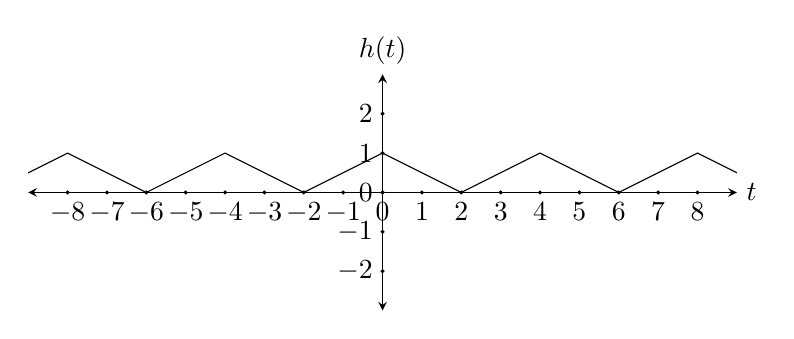
\begin{tikzpicture}[scale = 0.5]
					\def\xMIN{-9};
					\def\xMAX{9};
					\def\yMIN{-3};
					\def\yMAX{3};

					\begin{scope}[stealth-stealth]
						\draw (\xMIN,0) -- (\xMAX,0) node [right] {$t$};
						\draw (0,\yMIN) -- (0,\yMAX) node [above] {$h(t)$};
					\end{scope}

					\begin{scope}
						\clip (\xMIN,\yMIN) rectangle (\xMAX,\yMAX);
						\draw[xshift = -8cm] (-2,0) -- (0,1) -- (2,0);
						\draw[xshift = -4cm] (-2,0) -- (0,1) -- (2,0);
						\draw[xshift = 0] (-2,0) -- (0,1) -- (2,0);
						\draw[xshift = 4cm] (-2,0) -- (0,1) -- (2,0);
						\draw[xshift = 8cm] (-2,0) -- (0,1) -- (2,0);
					\end{scope}

					\begin{scope}
						\foreach \x in {-8,...,8}
						{
							\filldraw (\x,0) circle (1pt) node [below] {$\x$};
						}

						\foreach \y in {-2,...,2}
						{
							\filldraw (0,\y) circle (1pt) node [left] {$\y$};
						}
					\end{scope}
				\end{tikzpicture}
			\end{figure}
		\item
			\begin{align*}
				T & = 3
			\end{align*}
			Therefore,
			\begin{align*}
				x(t) & = \sum\limits_{k = -\infty}^{\infty} \delta(t - 3 k)
			\end{align*}
			Therefore,
			\begin{align*}
				y(t) & = x(t) \ast h(t)                                               \\
                                     & = h(t) \ast \sum\limits_{k = -\infty}^{\infty} \delta(t - 3 k) \\
                                     & = \sum\limits_{k = -\infty}^{\infty} h(t - 3 k)
			\end{align*}
			\begin{figure}[H]
				\centering
				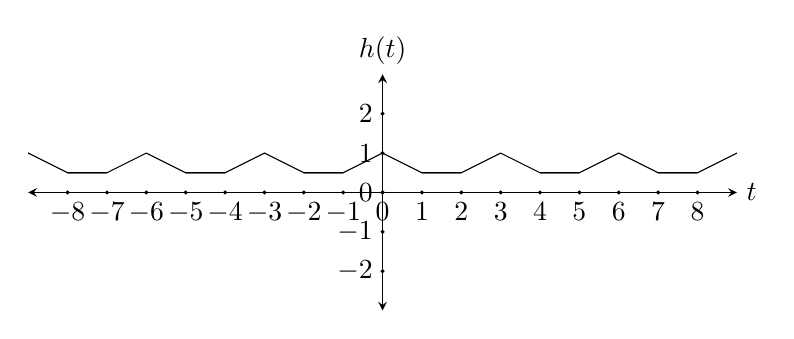
\begin{tikzpicture}[scale = 0.5]
					\def\xMIN{-9};
					\def\xMAX{9};
					\def\yMIN{-3};
					\def\yMAX{3};

					\begin{scope}[stealth-stealth]
						\draw (\xMIN,0) -- (\xMAX,0) node [right] {$t$};
						\draw (0,\yMIN) -- (0,\yMAX) node [above] {$h(t)$};
					\end{scope}

					\begin{scope}
						\clip (\xMIN,\yMIN) rectangle (\xMAX,\yMAX);
						\draw[xshift = -9cm] (-2,0.5) -- (-1,0.5) -- (0,1) -- (1,0.5) -- (2,0.5);
						\draw[xshift = -6cm] (-2,0.5) -- (-1,0.5) -- (0,1) -- (1,0.5) -- (2,0.5);
						\draw[xshift = -3cm] (-2,0.5) -- (-1,0.5) -- (0,1) -- (1,0.5) -- (2,0.5);
						\draw[xshift = 0] (-2,0.5) -- (-1,0.5) -- (0,1) -- (1,0.5) -- (2,0.5);
						\draw[xshift = 3cm] (-2,0.5) -- (-1,0.5) -- (0,1) -- (1,0.5) -- (2,0.5);
						\draw[xshift = 6cm] (-2,0.5) -- (-1,0.5) -- (0,1) -- (1,0.5) -- (2,0.5);
						\draw[xshift = 9cm] (-2,0.5) -- (-1,0.5) -- (0,1) -- (1,0.5) -- (2,0.5);
					\end{scope}

					\begin{scope}
						\foreach \x in {-8,...,8}
						{
							\filldraw (\x,0) circle (1pt) node [below] {$\x$};
						}

						\foreach \y in {-2,...,2}
						{
							\filldraw (0,\y) circle (1pt) node [left] {$\y$};
						}
					\end{scope}
				\end{tikzpicture}
			\end{figure}
		\item
			\begin{align*}
				T & = 1
			\end{align*}
			Therefore,
			\begin{align*}
				x(t) & = \sum\limits_{k = -\infty}^{\infty} \delta(t - k)
			\end{align*}
			Therefore,
			\begin{align*}
				y(t) & = x(t) \ast h(t)                                             \\
                                     & = h(t) \ast \sum\limits_{k = -\infty}^{\infty} \delta(t - k) \\
                                     & = \sum\limits_{k = -\infty}^{\infty} h(t - k)
			\end{align*}
			\begin{figure}[H]
				\centering
				\begin{tikzpicture}[scale = 0.5]
					\def\xMIN{-9};
					\def\xMAX{9};
					\def\yMIN{-3};
					\def\yMAX{3};

					\begin{scope}[stealth-stealth]
						\draw (\xMIN,0) -- (\xMAX,0) node [right] {$t$};
						\draw (0,\yMIN) -- (0,\yMAX) node [above] {$h(t)$};
					\end{scope}

					\begin{scope}
						\draw (\xMIN,2) -- (\xMAX,2);
					\end{scope}

					\begin{scope}
						\foreach \x in {-8,...,8}
						{
							\filldraw (\x,0) circle (1pt) node [below] {$\x$};
						}

						\foreach \y in {-2,...,2}
						{
							\filldraw (0,\y) circle (1pt) node [left] {$\y$};
						}
					\end{scope}
				\end{tikzpicture}
			\end{figure}
	\end{enumerate}
\end{solution}

\begin{question}
	Consider the following RC circuit.
	\begin{figure}[H]
		\centering
		\includegraphics[width = 0.8\textwidth]{./plot3.pdf}
	\end{figure}
	\begin{enumerate}
		\item
			Using Kirchoff's Laws, find a differential equation of the voltage of the capacitor $y(t)$, as a function of the original voltage $x(t)$.
		\item
			Under the assumption of initial time $-\infty$, solve the differential equation.
			The solution should be represented as an integral that depends on the input $x(t)$.
		\item
			Find the impulse response.
		\item
			Find the unit step response.
		\item
			Find the frequency response and draw the phase and amplitude of the system.
			Is it HP/BP/LP?
		\item
			Derive the frequency response from voltage division considerations using impedances.
	\end{enumerate}
\end{question}

\begin{solution}
	\begin{enumerate}[leftmargin=*]
		\item
			\begin{align*}
				y(t)                                  & = x(t) - i(t) R            \\
				\therefore y(t)                       & = x(t) - R C \dod{y(t)}{t} \\
				\therefore y'(t) + \frac{1}{R C} y(t) & = \frac{1}{R C} x(t)       \\
			\end{align*}
		\item
			\begin{align*}
				y'(t) + \frac{1}{R C} y(t) & = \frac{1}{R C} x(t)
			\end{align*}
			Therefore, the integrating factor is
			\begin{align*}
				\mu(t) & = e^{\int \frac{1}{R C} \dif t} \\
                                       & = e^{\frac{t}{R C}}
			\end{align*}
			Therefore,
			\begin{align*}
				y(t) & = \frac{1}{\mu(t)} \int\limits_{-\infty}^{t} \mu(t) \frac{1}{R C} x(t) \dif t \\
                                     & = \frac{e^{-\frac{t}{R C}}}{R C} \int\limits_{-\infty}^{t} e^{\frac{t}{R C}} x(t) \dif t
			\end{align*}
		\item
			\begin{align*}
				h(t) & = \frac{e^{-\frac{t}{R C}}}{R C} \int\limits_{-\infty}^{t} e^{\frac{t}{R C}} x(t) \dif t      \\
                                     & = \frac{e^{-\frac{t}{R C}}}{R C} \int\limits_{-\infty}^{t} e^{\frac{t}{R C}} \delta(t) \dif t \\
                                     & = \frac{e^{-\frac{t}{R C}}}{R C} e^{0}                                                        \\
                                     & = \frac{e^{-\frac{t}{R C}}}{R C}
			\end{align*}
		\item
			Let
			\begin{align*}
				x(t) & = u(t)
			\end{align*}
			Therefore,
			\begin{align*}
				y(t) & = \int\limits_{0}^{t} h(t) \dif t                            \\
                                     & = \int\limits_{0}^{t} \frac{e^{-\frac{t}{R C}}}{R C}         \\
                                     & = \left. -\frac{e^{-\frac{t}{R C}}}{R^2 C^2} \right|_{0}^{t} \\
                                     & = \frac{1 + e^{-\frac{t}{R C}}}{R^2 C^2}
			\end{align*}
		\item
			\begin{align*}
				H(s) & = \mathcal{L}\left\{ h(t) \right\}                           \\
                                     & = \mathcal{L}\left\{ \frac{e^{-\frac{t}{R C}}}{R C} \right\} \\
                                     & = \frac{1}{1 + R C s}
			\end{align*}
			\begin{figure}[H]
				\centering
				\includegraphics[width = 0.8\textwidth]{./plot1.pdf}
			\end{figure}
			Therefore, it is a low pass filter.
		\item
			\begin{align*}
				X(s)            & = I(s) R + Y(s)                                           \\
                                                & = s Y(s) C R + Y(s)                                       \\
				\therefore Y(s) & = \frac{X(s)}{1 + s C R}                                  \\
                                                & = \frac{\mathcal{L}\left\{ \delta(t) \right\}}{1 + s C R} \\
                                                & = \frac{1}{1 + s C R}
			\end{align*}
	\end{enumerate}
\end{solution}

\begin{question}
	Given
	\begin{align*}
		x[n] = a^n u[n] \\
		h[n] = u[n]
	\end{align*}
	Find $y[n]$ using convolution.
\end{question}

\begin{solution}
	\begin{align*}
		y[n] & = x[n] \ast h[n]                                       \\
                     & = \sum\limits_{k = -\infty}^{\infty} x[k] h[n - k]     \\
                     & = \sum\limits_{k = -\infty}^{\infty} a^k u[k] u[n - k] \\
                     & = \sum\limits_{k = -\infty}^{n} a^k u[k]               \\
                     & = \sum\limits_{k = 0}^{n} a^k                          \\
	\end{align*}
\end{solution}

\begin{question}
	For each of the following signals, determine whether it is an energy signal or a power signal.
	In case the signal is an energy signal, calculate the energy.
	In case the signal is a power signal, calculate the average power.
	\begin{enumerate}
		\item
			$
				x(t) =
					\begin{cases}
						t &;\quad 0 \le t \le 1\\
						2 - t &;\quad 1 \le t \le 2\\
						0 &;\quad \text{otherwise}\\
					\end{cases}
			$
		\item
			$
				x[n] =
					\begin{cases}
						n &;\quad 0 \le t \le 5\\
						10 - n &;\quad 5 \le t \le 10\\
						0 &;\quad \text{otherwise}\\
					\end{cases}
			$
		\item
			$x(t) = 5 \cos(\pi t) + \sin(5 \pi t)$, $-\infty < t < \infty$
		\item
			$
				x(t) =
					\begin{cases}
						5 \cos(\pi t) &;\quad -1 \le t \le 1\\
						0 &;\quad \text{otherwise}\\
					\end{cases}
			$
		\item
			$
				x(t) =
					\begin{cases}
						5 \cos(\pi t) &;\quad -0.5 \le t \le 0.5\\
						0 &;\quad \text{otherwise}\\
					\end{cases}
			$
		\item
			$
				x[n] =
					\begin{cases}
						\sin(\pi n) &;\quad -4 \le n \le 4\\
						0 &;\quad \text{otherwise}\\
					\end{cases}
			$
		\item
			$
				x[n] =
					\begin{cases}
						\cos(\pi n) &;\quad -4 \le n \le 4\\
						0 &;\quad \text{otherwise}\\
					\end{cases}
			$
		\item
			$
				x[n] =
					\begin{cases}
						\cos(\pi n) &;\quad 0 \le n\\
						0 &;\quad \text{otherwise}\\
					\end{cases}
			$
	\end{enumerate}
\end{question}

\begin{solution}
	\begin{enumerate}[leftmargin=*]
		\item
			\begin{align*}
				E_{\infty} & = \lim\limits_{T \to \infty} \int\limits_{-T}^{T} \left| x(t) \right|^2 \dif t                                                        \\
                                           & = \lim\limits_{T \to \infty} \left( \int\limits_{0}^{1} t^2 \dif t + \int\limits_{1}^{2} (2 - t)^2 \dif t \right)                     \\
                                           & = \lim\limits_{T \to \infty} \left( \left. \frac{t^3}{3} \right|_{0}^{1} + \left. 4 t - 2 t^2 + \frac{t^3}{2} \right|_{1}^{2} \right) \\
                                           & = \lim\limits_{T \to \infty} \left( \frac{1}{3} + 8 - 8 + \frac{8}{2} - 4 + 2 - \frac{1}{2} \right)                                   \\
                                           & = \lim\limits_{T \to \infty} \left( \frac{11}{6} \right)                                                                              \\
                                           & = \frac{11}{6}
			\end{align*}
			Therefore, as $E_{\infty}$ is finite, the signal is an energy signal.
		\item
			\begin{align*}
				E_{\infty} & = \lim\limits_{N \to \infty} \sum\limits_{n = -N}^{N} \left| x[n] \right|^2                    \\
                                           & = \lim\limits_{N \to \infty} \sum\limits_{n = 0}^{5} n^2 + \sum\limits_{n = 6}^{10} (10 - n)^2 \\
                                           & = \lim\limits_{N \to \infty} 85                                                                \\
                                           & = 85
			\end{align*}
			Therefore, as $E_{\infty}$ is finite, the signal is an energy signal.
		\item
			\begin{align*}
				E_{\infty} & = \lim\limits_{T \to \infty} \int\limits_{-T}^{T} \left| x(t) \right|^2 \dif t                                                        \\
                                           & = \lim\limits_{T \to \infty} \int\limits_{-T}^{T} \left| 5 \cos(5 t) + \sin(5 \pi t) \right|^2 \dif t                                 \\
                                           & = \lim\limits_{T \to \infty} \int\limits_{-T}^{T} \left( 25 \cos^2(5 t) + 10 \cos(5 t) \sin(5 \pi t) + \sin^2(5 \pi t) \right) \dif t \\
                                           & = \lim\limits_{T \to \infty} 26 T + \frac{5}{2} \sin(10 T) - \frac{\sin(10 \pi T)}{10 \pi}                                            \\
                                           & \to \infty
			\end{align*}
			Therefore, as $E_{\infty}$ is not finite, the signal is not an energy signal.
			\begin{align*}
				P_{\infty} & = \lim\limits_{T \to \infty} \frac{1}{2 T} \int\limits_{-T}^{T} \left| x(t) \right|^2 \dif t                                                        \\
                                           & = \lim\limits_{T \to \infty} \frac{1}{2 T} \int\limits_{-T}^{T} \left| 5 \cos(5 t) + \sin(5 \pi t) \right|^2 \dif t                                 \\
                                           & = \lim\limits_{T \to \infty} \frac{1}{2 T} \int\limits_{-T}^{T} \left( 25 \cos^2(5 t) + 10 \cos(5 t) \sin(5 \pi t) + \sin^2(5 \pi t) \right) \dif t \\
                                           & = \lim\limits_{T \to \infty} \frac{1}{2 T} \left( 26 T + \frac{5 \sin(10 T)}{2} - \frac{\sin(10 \pi T)}{10 \pi} \right)                             \\
                                           & = \lim\limits_{T \to \infty} 26 + \frac{5 \sin(10 T)}{2 T} - \frac{\sin(10 \pi T)}{10 \pi T}                                                        \\
                                           & = 26
			\end{align*}
			Therefore, as $P_{\infty}$ is finite, the signal is an power signal.
		\item
			\begin{align*}
				E_{\infty} & = \lim\limits_{T \to \infty} \int\limits_{-T}^{T} \left| x(t) \right|^2 \dif t \\
                                           & = \lim\limits_{T \to \infty} \int\limits_{-1}^{1} 25 \cos^2(\pi t) \dif t      \\
                                           & = 25
			\end{align*}
			Therefore, as $E_{\infty}$ is finite, the signal is an energy signal.
		\item
			\begin{align*}
				E_{\infty} & = \lim\limits_{T \to \infty} \int\limits_{-T}^{T} \left| x(t) \right|^2 \dif t \\
                                           & = \lim\limits_{T \to \infty} \int\limits_{-0.5}^{0.5} 25 \cos^2(\pi t) \dif t  \\
                                           & = \frac{25}{2}
			\end{align*}
			Therefore, as $E_{\infty}$ is finite, the signal is an energy signal.
		\item
			\begin{align*}
				E_{\infty} & = \lim\limits_{N \to \infty} \sum\limits_{n = -N}^{N} \left| x[n] \right|^2 \\
                                           & = \lim\limits_{N \to \infty} \sum\limits_{n = -4}^{4} \sin^2(n \pi)         \\
                                           & = \sum\limits_{n = -4}^{4} \sin^2(n \pi)                                    \\
                                           & = 0
			\end{align*}
			Therefore, as $E_{\infty}$ is finite, the signal is an energy signal.
		\item
			\begin{align*}
				E_{\infty} & = \lim\limits_{N \to \infty} \sum\limits_{n = -N}^{N} \left| x[n] \right|^2 \\
                                           & = \lim\limits_{N \to \infty} \sum\limits_{n = -4}^{4} \cos^2(n \pi)         \\
                                           & = \sum\limits_{n = -4}^{4} \cos^2(n \pi)                                    \\
                                           & = 9
			\end{align*}
			Therefore, as $E_{\infty}$ is finite, the signal is an energy signal.
		\item
			\begin{align*}
				E_{\infty} & = \lim\limits_{N \to \infty} \sum\limits_{n = -N}^{N} \left| x[n] \right|^2 \\
                                           & = \lim\limits_{N \to \infty} \sum\limits_{n = 0}^{N} \cos^2(n \pi)          \\
                                           & = \lim\limits_{N \to \infty} \sum\limits_{n = 0}^{N} \cos^2(n \pi)          \\
                                           & = \lim\limits_{N \to \infty} \sum\limits_{n = 0}^{N} 1                      \\
                                           & = \lim\limits_{N \to \infty} N + 1                                          \\
                                           & \to \infty
			\end{align*}
			Therefore, as $E_{\infty}$ is not finite, the signal is not an energy signal.
			\begin{align*}
				P_{\infty} & = \lim\limits_{N \to \infty} \frac{1}{2 N + 1} \sum\limits_{n = -N}^{N} \left| x[n] \right|^2 \\
                                           & = \lim\limits_{N \to \infty} \frac{1}{2 N + 1} \sum\limits_{n = 0}^{N} \cos^2(n \pi)          \\
                                           & = \lim\limits_{N \to \infty} \frac{1}{2 N + 1} \sum\limits_{n = 0}^{N} 1                      \\
                                           & = \lim\limits_{N \to \infty} \frac{N + 1}{2 N + 1}                                            \\
                                           & = \lim\limits_{N \to \infty} \frac{1 + \frac{1}{N}}{2 + \frac{1}{N}}                          \\
                                           & = \frac{1}{2}
			\end{align*}
			Therefore, as $P_{\infty}$ is finite, the signal is an power signal.
	\end{enumerate}
\end{solution}

\end{document}
